\documentclass[11pt]{article}
\usepackage[utf8]{inputenc}
\usepackage{dirtytalk}
\usepackage{mathrsfs}
\usepackage{blindtext}
\usepackage{csquotes}
\usepackage{mathtools} 	
\usepackage{polynom}
\usepackage{amsthm}
%for the rendering of maths
\numberwithin{equation}{section}					
%reset numbering within a structural object
\numberwithin{figure}{section}						
%reset numbering within a structural object
 \usepackage{natbib}
\usepackage[margin=1.5cm]{geometry}
\usepackage{url}
\usepackage{amssymb,amsmath,graphics}
\title{\textbf{Taller Introducción a la Teoría de Conjuntos\\ Propiedades de Ordinales}}
\author{}
\date{}


\begin{document}
\maketitle
\renewcommand\qedsymbol{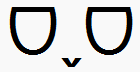
\includegraphics[height=2ex]{Demo face.png}}
Muestre las siguientes propiedades de los ordinales:
\begin{enumerate}
    \item Considere la colección $C$ de todos los ordinales, muestre que $<$ es un orden total en $C$.
    \begin{proof}[\textbf{Solución}]
    Para demostrar que la colección $C$ de ordinales es un orden total debemos mostrar que dados $\alpha$ y $\beta$ ordinales pertenecientes a $C$ siempre se tiene que $\alpha\in\beta$ ó $\alpha=\beta$ ó $\beta\in\alpha$.\\
    Sean $\alpha,\beta$ ordinales, $\alpha\cap\beta$ también es ordinal (esto fue demostrado en clase). Es evidente que $\alpha\cap\beta\subseteq\alpha$ y $\alpha\cap\beta\subseteq\beta$. Si $\alpha\cap\beta=\alpha$ quiere decir que $\alpha\subseteq\beta$, luego $\alpha\subset\beta$ ó $\alpha=\beta$ y por lo tanto $\alpha\in\beta$ ó $\alpha=\beta$. De manera análoga si se tiene que $\alpha\cap\beta=\beta$ se concluye que $\beta\in\alpha$ ó $\alpha=\beta$. Ahora solo falta considerar que ocurre si $\alpha\cap\beta\subset\alpha$ y $\alpha\cap\beta\subset\beta$ luego $\alpha\cap\beta\in\alpha$ y $\alpha\cap\beta\in\beta$ y por tanto $\alpha\cap\beta\in\alpha\cap\beta$ lo que es una contradicción para ordinales y por lo tanto no se puede tener este caso.\\
    De esta forma queda demostrado que las únicas posibilidades son que $\alpha\in\beta$ ó $\alpha=\beta$ ó $\beta\in\alpha$.
    \end{proof}
    \item Para todo ordinal $\alpha$, $\alpha=\{\beta:\beta<\alpha\}$.
    \begin{proof}[\textbf{Solución}]
    Para demostrar esto debemos mostrar que todo ordinal es un conjunto de ordinales.\\
    Tomemos $\beta\in\alpha$ ($\beta<\alpha$) primero probaremos que $\beta$ es transitivo. Sea $\gamma\in\beta$ queremos mostrar que $\gamma\subseteq\beta$. Primero note que como $\alpha$ es ordinal tenemos que $\beta\subseteq\alpha$ por lo tanto $\gamma\in\alpha$ y $\gamma\subseteq\alpha$, ahora tomando un $\zeta\in\gamma$ se tiene que $\zeta\in\alpha$, luego $\alpha$  al ser ordinal esta bien ordenado por $\in$ y además $\beta,\gamma,\zeta$ son elementos de $\alpha$, luego como se tiene que $\zeta\in\gamma$ y $\gamma\in\beta$ implicando que $\zeta\in\beta$, de esta forma demostrando que $\gamma\subseteq\beta$ y por lo tanto $\beta$ es transitivo.\\
    Ahora recordemos que $\beta\subseteq\alpha$, luego la relación $\in_\beta$ es una restricción de la relación $\in_\alpha$ por lo tanto como esta es un buen orden entonces $\in_\beta$ también es un buen orden probando de esta forma que $\beta$ es un ordinal y por lo tanto se demuestra la propiedad.
    \end{proof}
    \item Si $\tilde{C}$ es una colección no vacía de ordinales, entonces $\bigcap\tilde{C}$ es un ordinal.
    \begin{proof}[\textbf{Solución}]
    Primero mostraremos la transitividad. Considere $x\in\bigcap\tilde{C}$ por definición como $\tilde{C}\neq\emptyset$ se tiene que $x\in\alpha$ para todo ordinal $\alpha\in\tilde{C}$, luego $x\subseteq\alpha$ para todo ordinal $\alpha\in\tilde{C}$ y por lo tanto $x\subseteq\tilde{C}$.\\
    Ahora para mostrar que $\bigcap\tilde{C}$ esta bien ordenado por $\in$, tomemos $x,y\in\bigcap\tilde{C}$ luego $x,y$ pertenecen a todo ordinal en $\tilde{C}$ particularmente pertenecen a $\beta\in\tilde{C}$. Como $x,y\in\beta$ y este es ordinal se tiene que $x\in y$ ó $x=y$ ó $y\in x$, luego como $x,y$ son arbitrarios esto se sostiene para cualquier $x,y\in\bigcap\tilde{C}$ y por tanto esta linealmente ordenado.\\
    Para el buen orden considere $A\neq\emptyset$ y $A\subseteq\bigcap\tilde{C}$, es sencillo notar que $A\subseteq\alpha$ para todo $\alpha\in\tilde{C}$ como $\alpha$ es un ordinal y $A\subseteq\alpha$, $A$ tiene elemento mínimo, Como $A$ es un subconjunto no vacío arbitrario se cumple que para todo $A\subseteq\bigcap\tilde{C}$, $A$ posee mínimo de esta forma demostrando el buen orden y por tanto concluyendo finalmente que $\bigcap\tilde{C}$ es un ordinal.
    \end{proof}
    \item Si $X$ es un conjunto no vacío de ordinales, entonces $\bigcup X$ es un ordinal y $\bigcup X=\textbf{sup}X$.
    \begin{proof}[\textbf{Solución}]
    Primero probemos que $\bigcup X$ es transitivo. Sea $x\in\bigcup X$ luego $x\in\alpha$ para algún $\alpha\in X$, como $\alpha$ es ordinal se tiene que $x\subseteq\alpha$ y como $\alpha\subseteq\bigcup X$, entonces $x\subseteq\bigcup X$.\\
    Ahora para mostrar que esta linealmente ordenado considere $x,y\in\bigcup X$ luego existen $\alpha,\beta\in\ X$ tales que $x\in\alpha$ y $y\in\beta$, luego sabemos que siempre se tiene que $\alpha\in\beta$ ó $\alpha=\beta$ ó $\beta\in\alpha$ luego sin perdida de generalidad asumamos que tenemos $\alpha\in\beta$, como $\beta$ es ordinal $\alpha\subseteq\beta$ y por tanto se tiene que $x,y\in\beta$ luego como $\beta$ esta linealmente ordenado entonces se tiene que $x\in y$ ó $x=y$ ó $y\in x$ y como eran arbitrarios se cumple para todos los $x,y\in\bigcup X$.\\
    Para el buen orden tomemos $A\subseteq\bigcup X$ no vacío, note que existe un $\alpha\in X$ tal que $A\cap\alpha\neq\emptyset$, note que como $\alpha$ es bien ordenado $A\cap\alpha$ tiene elemento mínimo, llamémoslo $a$, ahora suponga que $a$ no es mínimo de $A$, considere $b=\textbf{min}A$ eso quiere decir que $b\in a$ y como $a\in\alpha$, $a\subseteq\alpha$ por lo tanto $b\in\alpha$ y $b\in A\cap\alpha$, pero esto contradice  el hecho de que $a$ es el mínimo de $A\cap\alpha$ por lo tanto $a=\textbf{min}A$, concluyendo de esta forma que $\bigcup X$ es ordinal.\\
    Por ultimo llamemos $\alpha:=\bigcup X$ y consideremos un $\zeta\in X$ arbitrario, luego note que $\zeta\subseteq\alpha$ entonces se tiene que $\zeta\subset\alpha$ o $\zeta=\alpha$, si $\zeta\subset\alpha$ entonces $\zeta\in\alpha$ mostrando que $\alpha$ es cota superior. Ahora considere un ordinal $\theta$ tal que para todo $\zeta\in X$ se tiene que $\zeta\in\theta$, luego $\zeta\subset\theta$ y por lo tanto $\alpha\subset\theta$ entonces $\alpha\in\theta$ mostrando que $\alpha$ es la menor cota superior y por lo tanto $\bigcup X=\alpha=\textbf{sup}X$.
    
    \end{proof}
    \item Para todo $\alpha$ ordinal, $\alpha\cup\{\alpha\}$ es un ordinal y $\alpha\cup\{\alpha\}=\textbf{inf}\{\beta:\beta>\alpha\}$.
    \begin{proof}[\textbf{Solución}]
    Primero para ver que es transitivo tomemos $x\in\alpha\cup\{\alpha\}$ luego $x\in\alpha$ o $x\in\{\alpha\}$, si $x\in\alpha$ como $\alpha$ es ordinal $x\subseteq\alpha$ y $x\subseteq\alpha\cup\{\alpha\}$, en caso de que $x\in\{\alpha\}$, $x=\alpha$ y es evidente que $x\subseteq\alpha$ y por tanto $x\subseteq\alpha\cup\{\alpha\}$.\\
    Para el orden lineal tomemos $x,y\in\alpha\cup\{\alpha\}$ luego $x,y\in\alpha$ o $x,y\in\{\alpha\}$, en el caso de que $x,y\in\alpha$ ya se tiene el orden lineal debido a que $\alpha$ es ordinal, en caso de que se tuviera que $x,y\in\{\alpha\}$ solo se puede tener que $x=y=\alpha$ igualmente pueden seguir siendo comparados, por ultimo sin perdida de generalidad si tenemos que $x\in\alpha$ y $y\in\{\alpha\}$ tenemos que $y=\alpha$ y por tanto $x\in y$ y por tanto se cumple que es orden lineal.\\
    Ahora para el buen orden considere $A\subseteq\alpha\cup\{\alpha\}$ no vacío, note que podemos considerar dos casos, cuando $A\subseteq\alpha$ o $A\subseteq\{\alpha\}$, si $A\subseteq\alpha$ se tiene que $A$ tiene mínimo ya que $\alpha$ es ordinal, si $A\subseteq\{\alpha\}$ note que $A=\emptyset$ o $A=\alpha$ en ambos casos tiene elemento mínimo por tanto esta bien ordenado.\\
    Hemos concluido que efectivamente $\alpha\cup\{\alpha\}$ es un ordinal ahora para ver que es el $\textbf{inf}\{\beta:\beta>\alpha\}$ note que $\alpha\in\alpha\cup\{\alpha\}$ entonces $\alpha\cup\{\alpha\}\in\textbf{inf}\{\beta:\beta>\alpha\}$, note ahora que para todo $k\in\textbf{inf}\{\beta:\beta>\alpha\}$ se tiene que $\alpha\cup\{\alpha\}\leq k$ y de esta forma concluimos que $\alpha\cup\{\alpha\}=\textbf{inf}\{\beta:\beta>\alpha\}$.
    \end{proof}
    \item Muestre que $C$ no es conjunto.
    \begin{proof}[\textbf{Solución}]
    Suponga que $C$ es conjunto, considere $\alpha\in\beta\in C$ como $\beta\in C$ quiere decir que es ordinal luego $\alpha$ también es ordinal y por tanto $\alpha\in C$ por lo tanto es transitivo y por un teorema todo conjunto de ordinales esta bien ordenado bajo $\in$ por lo tanto $C$ es un ordinal, pero como $C$ es el conjunto de todos los ordinales se debe de tener que $C\in C$ lo cual no se tiene para ordinales, contradicción. Así se concluye que $C$ no es conjunto.
    \end{proof}
    \item Muestre que la relación $(A,<_A)$ es isomorfo a $(B,<_B)$ es de equivalencia en conjuntos ordenados.
    \begin{proof}[\textbf{Solución}]
    Para mostrar que es una relación de equivalencia hay que ver si se tiene que la relación es i.Reflexiva, ii.Simétrica y iii.Transitiva:
    \begin{itemize}
        \item[i.]Note que existe el isomorfismo entre $(A,<_A)$ y si mismo por medio de $f:A\longrightarrow A$ siendo $f$ la identidad, particularmente llamado automorfismo.
        \item[ii.]Si $(A,<_A)$ es isomorfo a $(B,<_B)$ quiere decir que el morfismo de orden $f:A\longrightarrow B$ es biyectiva y que $f^{-1}$ es un morfismo de orden, luego como $f$ es biyectiva, $f^{-1}:B\longrightarrow A$ es biyectiva y por lo tanto $(B,<_B)$ es isomorfo a $(A,<_A)$.
        \item[iii.]Si Si $(A,<_A)$ es isomorfo a $(B,<_B)$ y si $(B,<_B)$ es isomorfo a $(C,<_C)$ quiere decir que los morfismos de orden $f:A\longrightarrow B$ y $g:B\longrightarrow C$ son biyectivas luego note que $g\circ f:A\longrightarrow C$ es biyectiva y es morfismo de orden por lo tanto Si $(A,<_A)$ es isomorfo a $(C,<_C)$.
    \end{itemize}
    De esta forma como probamos las 3 propiedades concluimos que el isomorfismo en conjuntos ordenados es una relación de equivalencia.
    \end{proof}
    \item Muestre que $\alpha$ es un ordinal limite si y solo si $\beta<\alpha$ implica que $\beta\cup\{\beta\}<\alpha$.
    \begin{proof}[\textbf{Solución}]
    ($\Rightarrow$) Como $\alpha$ es ordinal limite, por definición esto es que $\alpha=\textbf{sup}\{\beta:\beta<\alpha\}$, sabemos que $\beta<\alpha$ por lo que consideraremos que ocurre con $\beta\cup\{\beta\}$. Note que $\beta\cup\{\beta\}\leq\alpha$, en caso de que $\beta\cup\{\beta\}=\alpha$ seria una contradicción ya que $\alpha$ es ordinal limite y por tanto no puede ser sucesor de nadie, de esta forma se debe de tener que $\beta\cup\{\beta\}<\alpha$.\\
    ($\Leftarrow$) Suponga que $\alpha$ no es ordinal limite, eso quiere decir que $\alpha=\zeta\cup\{\zeta\}$ con $\zeta$ un ordinal, notemos que $\zeta<\alpha$ por lo que por hipótesis $\zeta\cup\{\zeta\}<\alpha=\zeta\cup\{\zeta\}$ una contradicción por lo tanto $\alpha$ debe de ser ordinal limite.
    \end{proof}
    \item Muestre que si $(A,<_A)$ es bien ordenado entonces no existen sucesiones estrictamente decrecientes infinitas.
    \begin{proof}[\textbf{Solución}]
    Supongamos que dicha sucesión si existe, entonces sea $S:N\longrightarrow A$ tal que $S(i)=a_i$ generando la sucesión $\langle a_0,a_1,a_2,\dotsc\rangle$ con $a_0>a_1>a_2>\dotsc$\\
    Primero consideremos $\textbf{min}\langle a_0,a_1,a_2,\dotsc\rangle$, como esta es una sucesión decreciente infinita es fácil darse cuenta que esta no tendrá mínimo pero note que  $\langle a_0,a_1,a_2,\dotsc\rangle\subseteq A$ entonces se tendría que $(A,<_A)$ no esta bien ordenado, una contradicción por lo que tal sucesión no puede existir.
    \end{proof}
    \item Muestre que para todo ordinal $\alpha$ existe un ordinal limite $\beta$ tal que $\beta>\alpha$.
    \begin{proof}[\textbf{Solución}]
    Procederemos por inducción transfinita sobre $\alpha$.\\
    Note que para $\alpha=0$ se tiene que $0<\omega$ y $\omega$ es ordinal limite por tanto verificamos que el caso base es valido.\\
   Supongamos que la propiedad se cumple para todo ordinal $\theta<\alpha$, ahora consideremos que pasa cuando $\alpha$ es sucesor de un ordinal, es decir $\alpha=\zeta+1>\zeta$. Notemos que como $\zeta<\alpha$ se tiene que existe un ordinal limite $\beta$ tal que $\zeta<\beta$, luego por la propiedad demostrada en el punto $8.$ se tiene que $\zeta+1<\beta$.\\
   Por ultimo consideremos el caso donde $\alpha$ es un ordinal limite, es decir $\alpha=\textbf{sup}\{\gamma:\gamma<\alpha\}$, note que para todo $\gamma$ se tiene que existe un ordinal limite $\beta$ tal que $\gamma<\beta$, luego se tiene que efectivamente $\textbf{sup}\{\gamma:\gamma<\alpha\}=\alpha<\beta$ por que de lo contrario $\beta\in\alpha$ y por lo tanto se tendría que $\beta\in\beta$ una contradicción.
    \end{proof}
    \item Muestre que para todo $\alpha,\beta,\gamma$ ordinales, en la aritmética ordinal se tiene que:
    \begin{itemize}
        \item[a)] $\alpha\cdot(\beta+\gamma)=\alpha\cdot\beta+\alpha\cdot\gamma$
        \item[b)] $\alpha^{\beta+\gamma}=\alpha^{\beta}\cdot\alpha^{\gamma}$
        \item[c)] $(\alpha^{\beta})^{\gamma}=\alpha^{(\beta\cdot\gamma)}$
    \end{itemize}
    \begin{proof}[\textbf{Solución}]
    Las tres siguientes propiedades serán demostradas usando inducción transfinita sobre $\gamma$.
    \begin{itemize}
        \item[a)] $\alpha\cdot(\beta+\gamma)=\alpha\cdot\beta+\alpha\cdot\gamma$
        \begin{proof}[\unskip\nopunct]
        \textbf{Caso base} $\gamma=0$\\
        Tenemos por definición de suma y de producto de ordinales que:
            \begin{equation*}
              \alpha\cdot(\beta+0)=\alpha\cdot\beta=\alpha\cdot\beta+0=\alpha\cdot\beta+\alpha\cdot0  
            \end{equation*}
        Verificando de esta forma el caso base.\\
        Supongamos que la propiedad se cumple para todo ordinal $\theta<\gamma$, ahora consideremos que pasa cuando $\gamma$ es sucesor de un ordinal, es decir $\gamma=\zeta+1>\zeta$.
        \begin{equation*}
        \alpha\cdot(\beta+(\zeta+1))=\alpha\cdot((\beta+\zeta)+1)=\alpha\cdot(\beta+\zeta)+\alpha=\alpha\cdot\beta+\alpha\cdot\zeta+\alpha=\alpha\cdot\beta+\alpha\cdot(\zeta+1)
        \end{equation*}
        Por ultimo consideremos el caso donde $\gamma$ es un ordinal limite y por tanto se tiene que:
        \begin{equation*}
        \alpha\cdot(\beta+\gamma)=\textbf{sup}\{\theta<\gamma:\alpha\cdot(\beta+\theta)\}=\textbf{sup}\{\theta<\gamma:\alpha\cdot\beta+\alpha\cdot\theta\}=\alpha\cdot\beta+\alpha\cdot\gamma    
        \end{equation*}
        De esta forma se prueba que la propiedad se cumple para todo ordinal.
        \end{proof}
        \item[b)] $\alpha^{\beta+\gamma}=\alpha^{\beta}\cdot\alpha^{\gamma}$
        \begin{proof}[\unskip\nopunct]
        \textbf{Caso base} $\gamma=0$\\
        Por las definiciones en aritmética ordinal tenemos que:
        \begin{equation*}
            \alpha^{\beta+0}=\alpha^\beta=\alpha^\beta\cdot1=\alpha^\beta\cdot\alpha^0
        \end{equation*}
        Verificando de esta forma el caso base.\\
        Supongamos que la propiedad se cumple para todo ordinal $\theta<\gamma$, ahora consideremos que pasa cuando $\gamma$ es sucesor de un ordinal, es decir $\gamma=\zeta+1>\zeta$.
        \begin{equation*}
            \alpha^{\beta+(\zeta+1)}=\alpha^{(\beta+\zeta)+1}=\alpha^{\beta+\zeta}\cdot\alpha=\alpha^\beta\cdot\alpha^\zeta\cdot\alpha=\alpha^\beta\cdot\alpha^{\zeta+1}
        \end{equation*}
        Por ultimo consideremos el caso donde $\gamma$ es un ordinal limite y por tanto se tiene que:
        \begin{equation*}
            \alpha^{\beta+\gamma}=\textbf{sup}\{\theta<\gamma:\alpha^{\beta+\theta}\}=\textbf{sup}\{\theta<\gamma:\alpha^\beta\cdot\alpha^\theta\}=\alpha^\beta\cdot\alpha^\gamma
        \end{equation*}
        De esta forma se prueba que la propiedad se cumple para todo ordinal.
        \end{proof}
        \item[c)] $(\alpha^{\beta})^{\gamma}=\alpha^{(\beta\cdot\gamma)}$\\
        \\
        \textbf{Caso base} $\gamma=0$\\
        Por las definiciones en aritmética ordinal tenemos que:
        \begin{equation*}
            (\alpha^\beta)^0=1=\alpha^0=\alpha^{\beta\cdot0}
        \end{equation*}
         Verificando de esta forma el caso base.\\
        Supongamos que la propiedad se cumple para todo ordinal $\theta<\gamma$, ahora consideremos que pasa cuando $\gamma$ es sucesor de un ordinal, es decir $\gamma=\zeta+1>\zeta$.
        \begin{equation*}
            (\alpha^\beta)^{\zeta+1}=(\alpha^\beta)^\zeta\cdot\alpha^\beta=\alpha^{\beta\cdot\zeta}\cdot\alpha^\beta=\alpha^{\beta\cdot\zeta+\beta}=\alpha^{\beta\cdot(\zeta+1)}
        \end{equation*}
         Por ultimo consideremos el caso donde $\gamma$ es un ordinal limite y por tanto se tiene que:
         \begin{equation*}
            (\alpha^\beta)^\gamma=\textbf{sup}\{\theta<\gamma:(\alpha^\beta)^\theta\}=\textbf{sup}\{\theta<\gamma:\alpha^{\beta\cdot\theta}\}=\alpha^{\beta\cdot\gamma} 
         \end{equation*}
    De esta forma se prueba que la propiedad se cumple para todo ordinal.
    \end{itemize}
    \end{proof}
    \item Muestre que si $\alpha<\beta$, ordinales, entonces $\alpha+\gamma\leq\beta+\gamma$, $\alpha\cdot\gamma\leq\beta\cdot\gamma$ y  $\alpha^\gamma\leq\beta^\gamma$.
    \begin{proof}[\textbf{Solución}]
    Al igual que en el ejercicio anterior se puede proceder por medio de inducción transfinita sobre $gamma$.
    \begin{itemize}
        \item[i.]$\alpha+\gamma\leq\beta+\gamma$
        \begin{proof}[\unskip\nopunct]
        \textbf{Caso base} $\gamma=0$
        \begin{equation*}
            \alpha+0=\alpha<\beta=\beta+0\Rightarrow\alpha+0\leq\beta+0
        \end{equation*}
        Verificando de esta forma el caso base.\\
        Supongamos que la propiedad se cumple para todo ordinal $\theta<\gamma$, ahora consideremos que pasa cuando $\gamma$ es sucesor de un ordinal, es decir $\gamma=\zeta+1>\zeta$.
        \begin{equation*}
            \alpha+(\zeta+1)=(\alpha+\zeta)+1\leq(\beta+\zeta)+1=\beta+(\zeta+1)
        \end{equation*}
        Por ultimo consideremos el caso donde $\gamma$ es ordinal limite, por definición:
        \begin{equation*}
            \alpha+\gamma=\textbf{sup}\{\theta<\gamma:\alpha+\theta\}
        \end{equation*}
        Ahora supongamos que $\beta+\gamma<\alpha+\gamma$, esto implica que no es cota superior de $\textbf{sup}\{\theta<\gamma:\alpha+\theta\}$ y por tanto existe $\zeta<\gamma$ tal que $\beta+\gamma<\alpha+\zeta$, luego tenemos que:
        \begin{equation*}
            \beta+\zeta\leq\textbf{sup}\{\delta<\gamma:\beta+\delta\}=\beta+\gamma<\alpha+\zeta\Rightarrow\beta+\zeta<\alpha+\zeta
        \end{equation*}
        Note que esto ultimo contradice la hipótesis de inducción por lo tanto se debe de tener que la propiedad también se cumple en este caso y por tanto para todo ordinal.
        \end{proof}
        \item[ii.]$\alpha\cdot\gamma\leq\beta\cdot\gamma$
        \begin{proof}[\unskip\nopunct]
        \textbf{Caso base} $\gamma=0$
        \begin{equation*}
            \alpha\cdot0=0=\beta\cdot0\Rightarrow\alpha\cdot0\leq\beta\cdot0
        \end{equation*}
        Verificando de esta forma el caso base.\\
        Supongamos que la propiedad se cumple para todo ordinal $\theta<\gamma$, ahora consideremos que pasa cuando $\gamma$ es sucesor de un ordinal, es decir $\gamma=\zeta+1>\zeta$.
        \begin{equation*}
            \alpha\cdot(\zeta+1)=\alpha\cdot\zeta+\alpha\leq\beta\cdot\zeta+\alpha<\beta\cdot\zeta+\beta=\beta\cdot(\zeta+1)\Rightarrow\alpha\cdot(\zeta+1)\leq\beta\cdot(\zeta+1)
        \end{equation*}
        Por ultimo consideremos el caso donde $\gamma$ es ordinal limite, por definición:
        \begin{equation*}
            \alpha\cdot\gamma=\textbf{sup}\{\theta<\gamma:\alpha\cdot\theta\}
        \end{equation*}
        Ahora supongamos que $\beta\cdot\gamma<\alpha\cdot\gamma$, esto implica que no es cota superior de $\textbf{sup}\{\theta<\gamma:\alpha\cdot\theta\}$ y por tanto existe $\zeta<\gamma$ tal que $\beta\cdot\gamma<\alpha\cdot\zeta$, luego tenemos que:
        \begin{equation*}
            \beta\cdot\zeta\leq\textbf{sup}\{\delta<\gamma:\beta\cdot\delta\}=\beta\cdot\gamma<\alpha\cdot\zeta\Rightarrow\beta\cdot\zeta<\alpha\cdot\zeta
        \end{equation*}
        Note que esto ultimo contradice la hipótesis de inducción por lo tanto se debe de tener que la propiedad también se cumple en este caso y por tanto para todo ordinal.
        \end{proof}
        \item[iii.]$\alpha^\gamma\leq\beta^\gamma$\\
        \\
        \textbf{Caso base} $\gamma=0$
        \begin{equation*}
            \alpha^0=1=\beta^0\Rightarrow\alpha^0\leq\beta^0
        \end{equation*}
        Verificando de esta forma el caso base.\\
        Supongamos que la propiedad se cumple para todo ordinal $\theta<\gamma$, ahora consideremos que pasa cuando $\gamma$ es sucesor de un ordinal, es decir $\gamma=\zeta+1>\zeta$.
        \begin{equation*}
            \alpha^{\zeta+1}=\alpha^\zeta\cdot\alpha\leq\beta^\zeta\cdot\alpha<\beta^\zeta\cdot\beta=\beta^{\zeta+1}\Rightarrow\alpha^{\zeta+1}\leq\beta^{\zeta+1}
        \end{equation*}
        Por ultimo consideremos el caso donde $\gamma$ es ordinal limite, por definición:
        \begin{equation*}
            \alpha^\gamma=\textbf{sup}\{\theta<\gamma:\alpha^\theta\}
        \end{equation*}
        Ahora supongamos que $\beta^\gamma<\alpha^\gamma$, esto implica que no es cota superior de $\textbf{sup}\{\theta<\gamma:\alpha^\theta\}$ y por tanto existe $\zeta<\gamma$ tal que $\beta^\gamma<\alpha^\zeta$, luego tenemos que:
        \begin{equation*}
            \beta^\zeta\leq\textbf{sup}\{\delta<\gamma:\beta^\delta\}=\beta^\gamma<\alpha^\zeta\Rightarrow\beta^\zeta<\alpha^\zeta
        \end{equation*}
        Note que esto ultimo contradice la hipótesis de inducción por lo tanto se debe de tener que la propiedad también se cumple en este caso y por tanto para todo ordinal.
    \end{itemize}
    \end{proof}
    \item Muestre que si $\alpha>0$, dado $\gamma$ ordinal, existe $\beta$ único y un $\rho$ único tal que $\rho<\alpha$ y $\gamma=\alpha\cdot\beta+\rho$.
    \begin{proof}[\textbf{Solución}]
    Comenzaremos esta demostración primero mostrando la existencia de $\beta,\rho$.\\
    Consideremos el caso donde $\gamma<\alpha$, luego $\beta=0$ y $\rho=\gamma$, note que se tiene la condición de que $\rho=\gamma<\alpha$ y luego también se tiene que $\alpha\cdot0+\gamma=\gamma$, mostrando la existencia.\\
    Ahora consideremos que ocurre cuando $\alpha\leq\gamma$, definamos $\beta=\bigcup\{\theta:\alpha\cdot\theta\leq\gamma\}$, notemos que $\{\theta:\alpha\cdot\theta\leq\gamma\}$ existe y no es vacío ya que $0\in\{\theta:\alpha\cdot\theta\leq\gamma\}$, note que por el ejercicio $4.$ podemos asegurar que $\beta$ es ordinal y además $\beta=\textbf{sup}\{\theta:\alpha\cdot\theta\leq\gamma\}$, Ahora como $\beta\neq\emptyset$ se tiene que tener que $\beta=\zeta+1$ o $\beta$ es ordinal limite.\\
    Suponga que $\beta=\zeta+1$ luego se tiene que $\zeta<\beta$ y $\alpha\cdot\zeta\leq\gamma$, además $\zeta<\theta$ para algún $\alpha\cdot\theta\leq\gamma$, note que $\theta<\beta$ ya que si fuera así $\zeta<\theta<\zeta+1$ una contradicción por tanto $\beta\leq\theta$ y por tanto $\alpha\cdot\beta\leq\gamma$.\\
    Ahora si $\beta$ es ordinal limite, note que para todo $\zeta\in\beta$ tal que $\alpha\cdot\zeta\leq\gamma$ se tiene que $\alpha\cdot\beta=\bigcup\limits_{\zeta\in\beta}(\alpha\cdot\zeta)\leq\bigcup\limits_{\zeta\in\beta}\gamma=\gamma$, de esta forma obtenemos en ambos casos que $\alpha\cdot\beta\leq\gamma$. Ahora supongamos que $\alpha\cdot(\beta+1)=\alpha\cdot\beta+\alpha\leq\gamma$, eso quiere decir que $\beta$ no es cota superior, una contradicción. Por lo tanto se debe tener que $\alpha\cdot\beta+\rho=\gamma$ para algún $\rho<\alpha$.
    Para concluir con la prueba mostraremos la unicidad de $\beta,\rho$. Suponga que tenemos que $\gamma=\alpha\cdot\beta_1+\rho_1$ para algún $\rho_1<\alpha$ y que $\gamma=\alpha\cdot\beta_2+\rho_2$ para algún $\rho_2<\alpha$, sabemos que para $\beta$ arbitrario tenemos que $\alpha\cdot\beta\leq\gamma<\alpha\cdot(\beta+1)$, luego entonces tenemos que $\alpha\cdot\beta_1<\alpha\cdot(\beta_2+1)$ y $\alpha\cdot\beta_2<\alpha\cdot(\beta_1+1)$ y por tanto se tiene que $\beta_1<\beta_2+1$ y $\beta_2<\beta_1+1$ luego esto es equivalente a tener que $\beta_1\leq\beta_2$ y $\beta_2\leq\beta_1$ por tanto $\beta_1=\beta_2$ mostrando de esa forma que $\beta,\rho$ deben de ser únicos ya que si $\beta$ es único $\rho$ también lo es.
    
    
    \end{proof}
\end{enumerate}

\end{document}
